\documentclass{standalone}
\input{../typography.tex.preamble}
\input{../tikz.tex.preamble}
\begin{document}
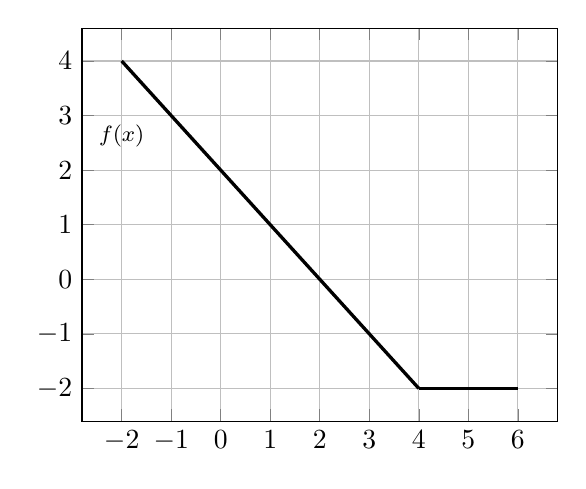
\begin{tikzpicture}
  \begin{axis}[width=3in,xtick={-2,-1,...,6}, ytick={-2,-1,...,4}, grid=both, minor tick num=0, enlargelimits]
    \addplot[very thick,black] coordinates {(-2, 4) (4,-2)};
    \addplot[very thick,black] coordinates {(4,-2) (6, -2)};
    \node[below] at (axis cs:-2,3) {\footnotesize \(f(x)\)};
  \end{axis}
\end{tikzpicture}
\end{document}
